\subsection{Obtained material and source distributions}

The audio branch contains 20 recordings from 14 publishing contexts, with median duration 66.15 minutes (range 28.05--109.92). Its actual media total is 1,691,458,021 bytes and 81,691.622 seconds. The common tokenizer yields 226,138 audio tokens and 13,556 written tokens; the original receipt totals remain 226,093 and 13,575 under their separate rules.

The current index describes 942 YouTube IDs and 362 literal routes, including 733 IDs selected under the current default collection policy. The distributions expose 180 publisher groups, 90 practitioner associations, 160 raw entity labels and 40 publisher-declared civilization labels with indexed material. Those association views overlap; none is a count of independently verified people or civilizations. Actual newly saved YouTube videos, caption tracks and bytes are all 0.

The logical storage plan contains 99 source artifacts and 1,703,635,307 bytes. The completed managed-local archive contains 200 independent copied files and 1,703,879,268 bytes, including 101 sidecar/manifest artifacts. Copies preserve the same observations. No Drive transfer, permanent external-retention guarantee or downloadable chat attachment is established by that local copy.

\subsection{Distinctive vocabulary and constructed topics}

The audio-wide mean TF--IDF vocabulary includes reality, physical, bashar, information, soul, idea, saying, change. Individual source vectors expose another layer: the Align records' top terms include protein, collagen and chocolate. Those are observable publishing/commercial vocabulary in the unsegmented transcript; treating all distinctive terms as attributed-message content would be unwarranted.

At the predeclared three-component display, seed-matched mean topic-term cosine is 0.864, with minimum 0.688. Higher stability at another component count does not identify a truer ontology. The components are labeled from their highest-weight terms in Table\ref{tab:topics}. The second component's workers/jumps/sole vocabulary is a source-inspection target, including possible recognition artifacts, rather than an independently validated conceptual category.

\begin{figure*}[t]
\centering
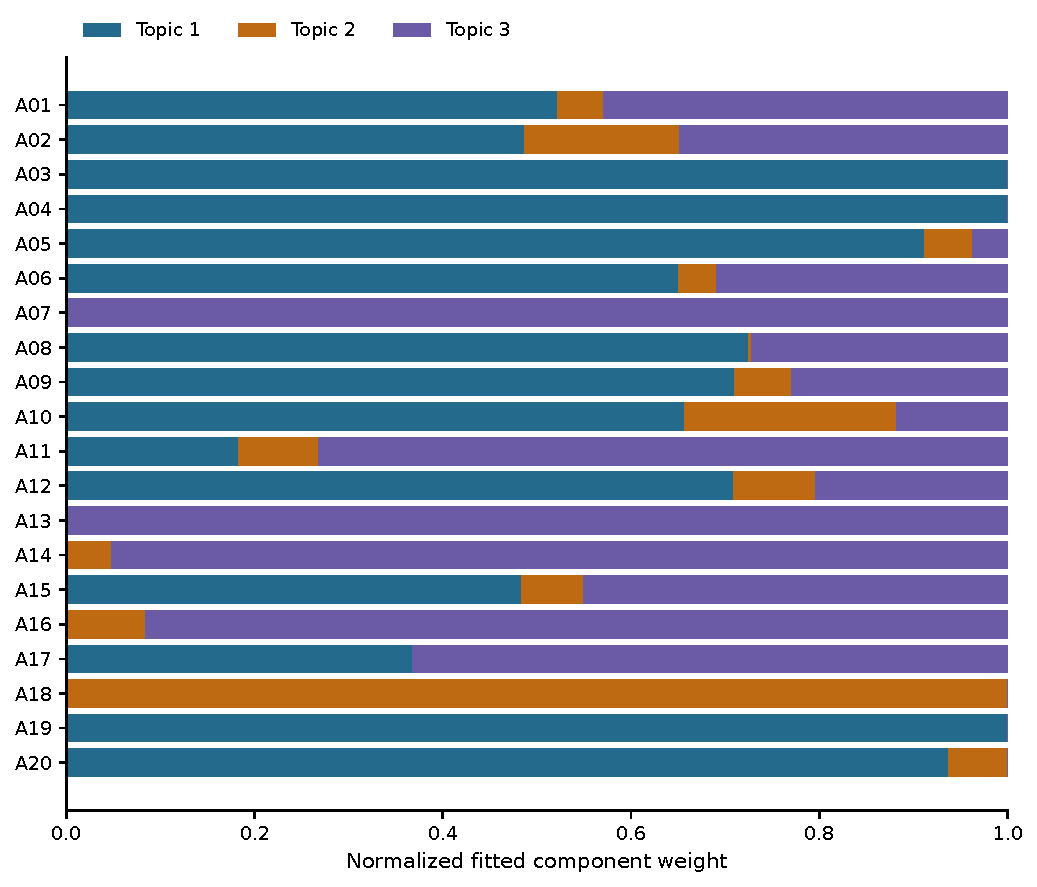
\includegraphics[width=\textwidth]{generated/figures/audio-topics.pdf}
\caption{NMF is fit to the 20 audio document vectors. Three display topics were selected prospectively for readable exploration; candidates 2--6 and seed-matched stability remain available. Weights sum to 1 per document. Top-term labels describe model components, not validated themes or distinct belief systems.}
\label{fig:audio-topics}
\end{figure*}


\begin{figure*}[t]
\centering
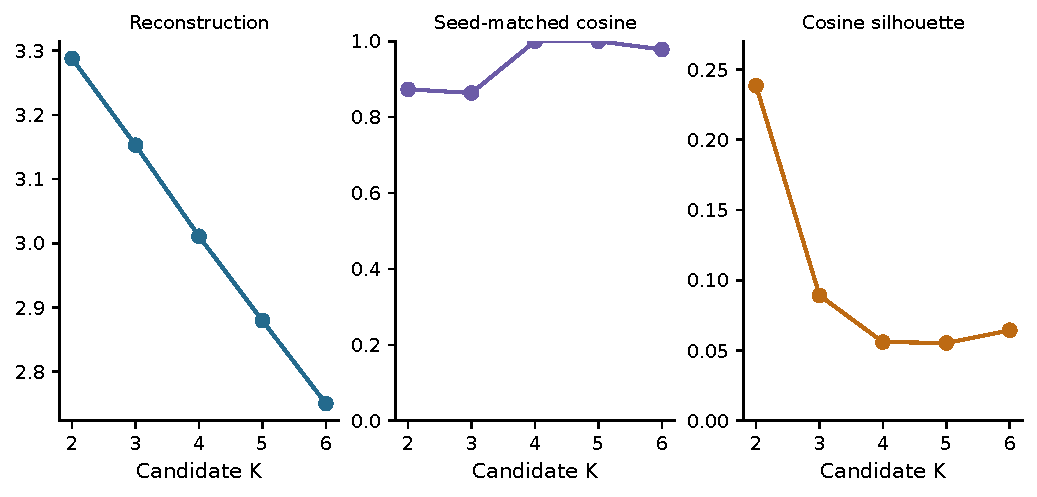
\includegraphics[width=\textwidth]{generated/figures/model-diagnostics.pdf}
\caption{NMF reconstruction decreases with model complexity and is not evidence that additional topics are substantively real. Topic stability is seed-matched term-vector cosine; KMeans selection exposes all candidate silhouettes. Neither stability nor a selected partition validates a medium or civilization ontology.}
\label{fig:model-diagnostics}
\end{figure*}


\subsection{Stable outlier partition and restricted overlays}

The selected K-means display uses K=2 and cosine silhouette 0.238. Its cluster sizes are nineteen and one: all nineteen Bashar-context recordings occupy one cluster, while the lone Athina record is the other. The cross-seed adjusted-Rand mean is 1.00. That numerical stability describes the same outlier partition. Source format, length, voice, vocabulary and context are confounded, so it cannot validate practitioner or civilization classes.

\begin{figure*}[t]
\centering
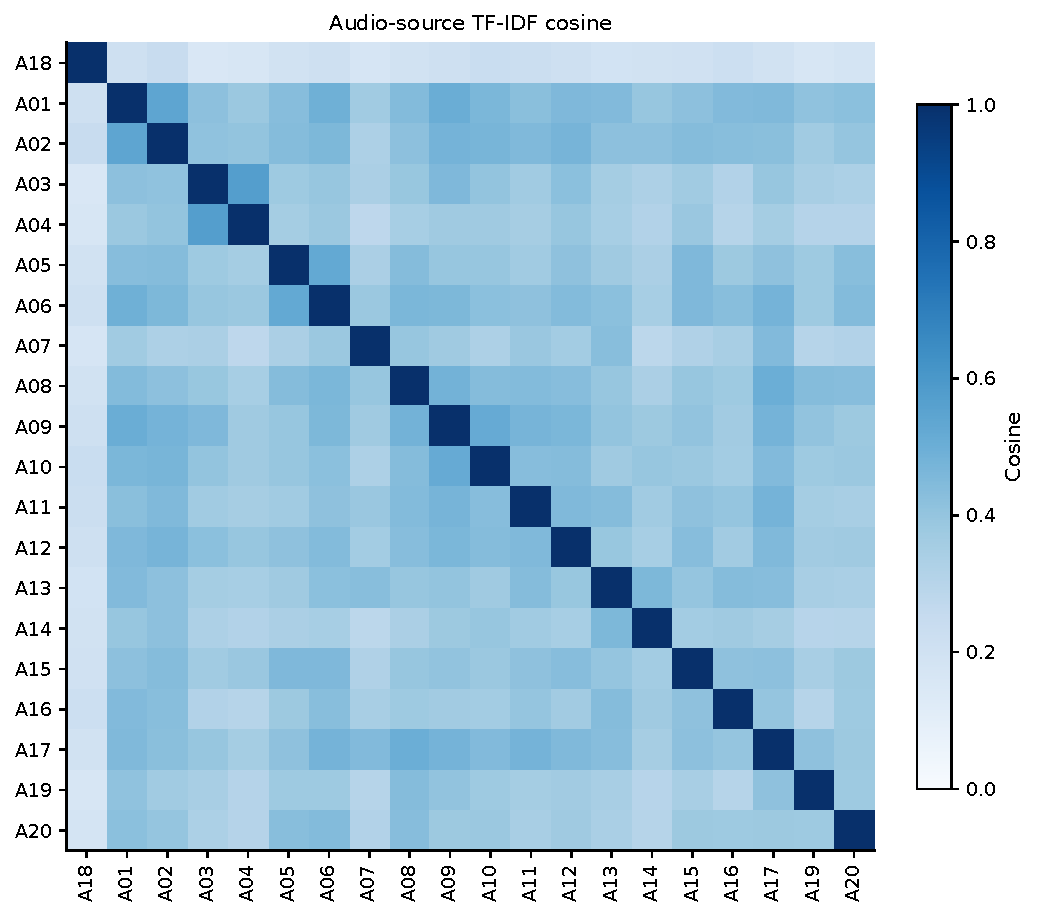
\includegraphics[width=\textwidth]{generated/figures/audio-cosine.pdf}
\caption{Cosine resemblance of 20 complete unverified ASR documents in a shared audio-only TF-IDF fit, ordered by the exploratory KMeans labels. Diagonal values are self-similarity. Short IDs join sources.json; resemblance is not semantic agreement, independent origin or a speaker comparison.}
\label{fig:audio-cosine}
\end{figure*}


\begin{figure*}[t]
\centering
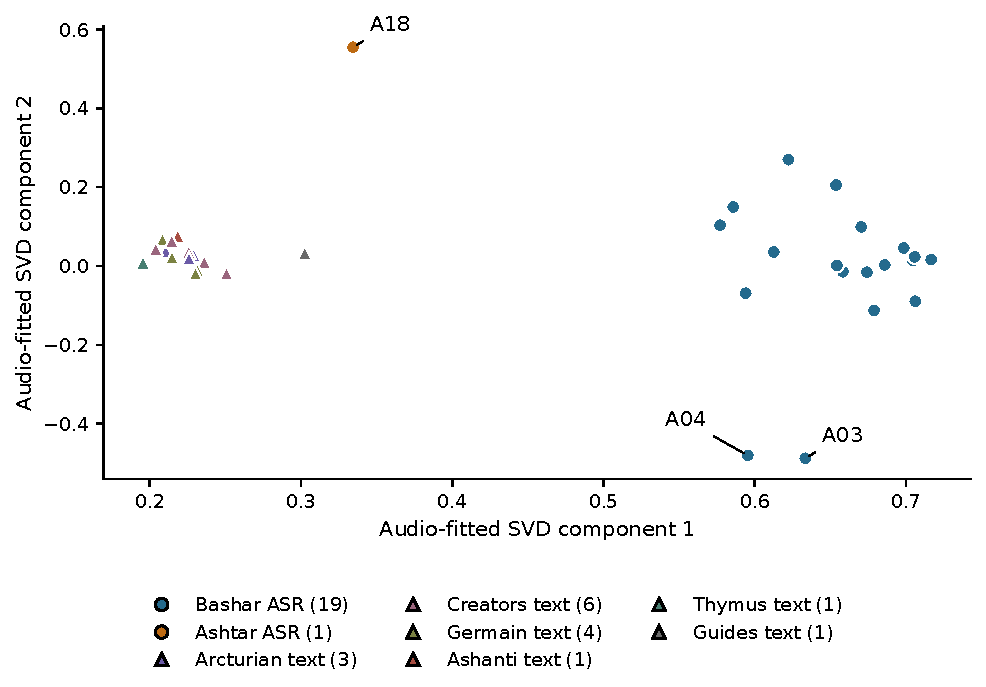
\includegraphics[width=\textwidth]{generated/figures/source-overlay.pdf}
\caption{Two-component SVD is fitted only to the 20 audio TF-IDF vectors; 16 written documents are projected through the same vocabulary and axes. Shapes distinguish modality and the short context key gives document counts. Only A03/A04 (retail-vocabulary examples) and A18 (the lone Ashtar source) are labeled to avoid crowding; all unchanged coordinates remain in analysis.json. Author, format, length and modality are confounded.}
\label{fig:source-overlay}
\end{figure*}


The two displayed SVD components explain 9.26 percent of the reported transformed-data variance. The projection is not a faithful map of every pairwise distance. Written points use the audio vocabulary and axes; they are comparison projections rather than evidence from a joint fit. The separate written NMF display is strongly shaped by author-attributed and publisher vocabulary, as its term table in the appendix shows.

The separately fitted written clustering selects K=6 by the same in-sample criterion, but its cosine silhouette is only 0.057. Cluster sizes are 3, 4, 3, 1, 4, 1. The Paul transcript and the one Thymus-labeled Daniel item are singleton clusters. This weak, source-confounded partition is not evidence for six substantive entity or civilization classes; all candidate scores are retained in the appendix.

\subsection{Lexical rates, mention graphs, and publication relations}

\begin{figure*}[t]
\centering
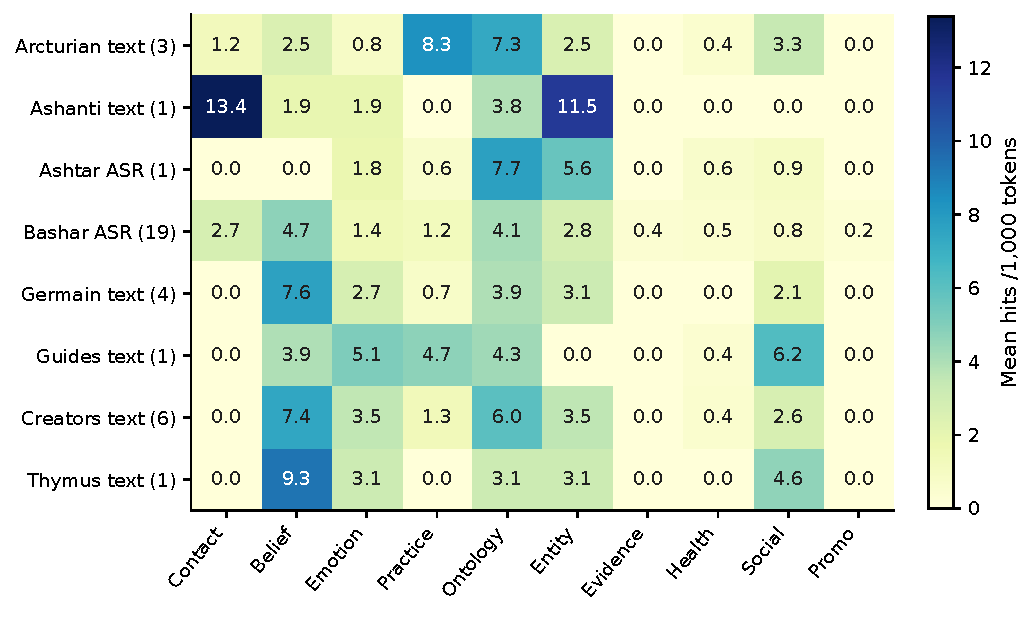
\includegraphics[width=\textwidth]{generated/figures/theme-overlay.pdf}
\caption{Overlapping predeclared keyword-family rates per 1000 common tokens, averaged equally across source documents within each labeled context. Counts are dictionary matches, not validated semantic coding. Source-attributed labels and modality are visible; singleton rows have no group-level uncertainty estimate. Promotion/footers and ASR error remain possible contributors.  Short headings follow the complete ten-family codebook order: contact/disclosure, belief/reality/agency, emotion/fear/self-worth, practice/enthusiasm/alignment, ontology/consciousness/dimensions, claimed-entity identity, epistemic validation/skepticism, health/healing, relationships/collective ethics, and commercial promotion.}
\label{fig:theme-overlay}
\end{figure*}


\begin{figure*}[t]
\centering
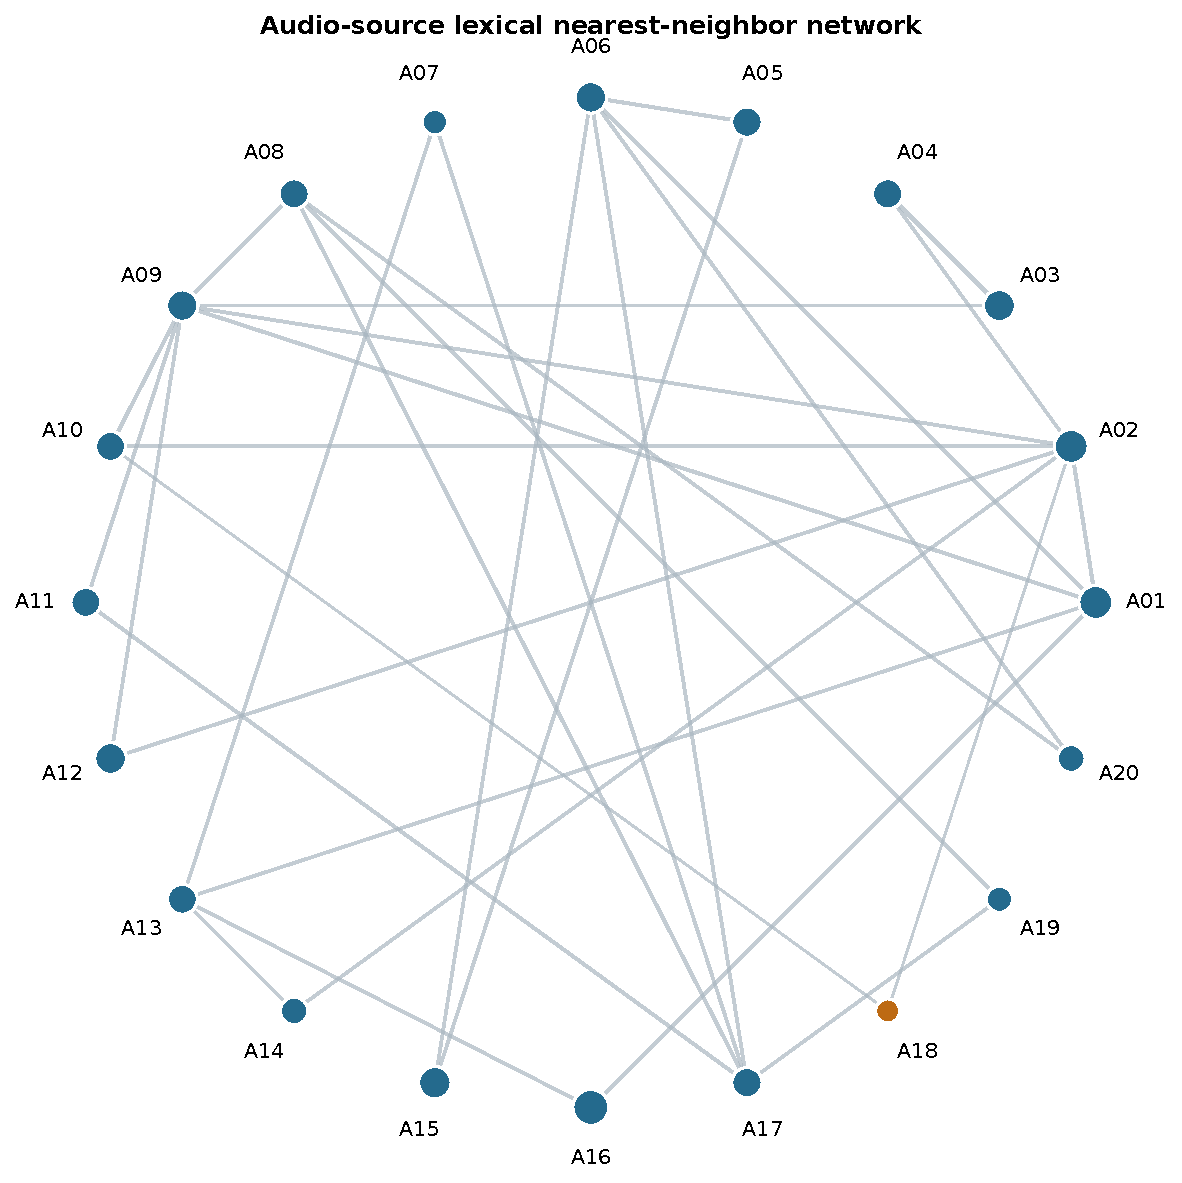
\includegraphics[width=\textwidth]{generated/figures/document-network.pdf}
\caption{Undirected union of each audio document's two nearest TF-IDF neighbors with cosine\(\geq\)0.20. Nodes are publication documents, sized by analytical token count; circular positions are purely schematic. Edges encode lexical resemblance, not social relations or independently shared ET knowledge. Threshold sensitivity is exported.}
\label{fig:document-network}
\end{figure*}


\begin{figure*}[t]
\centering
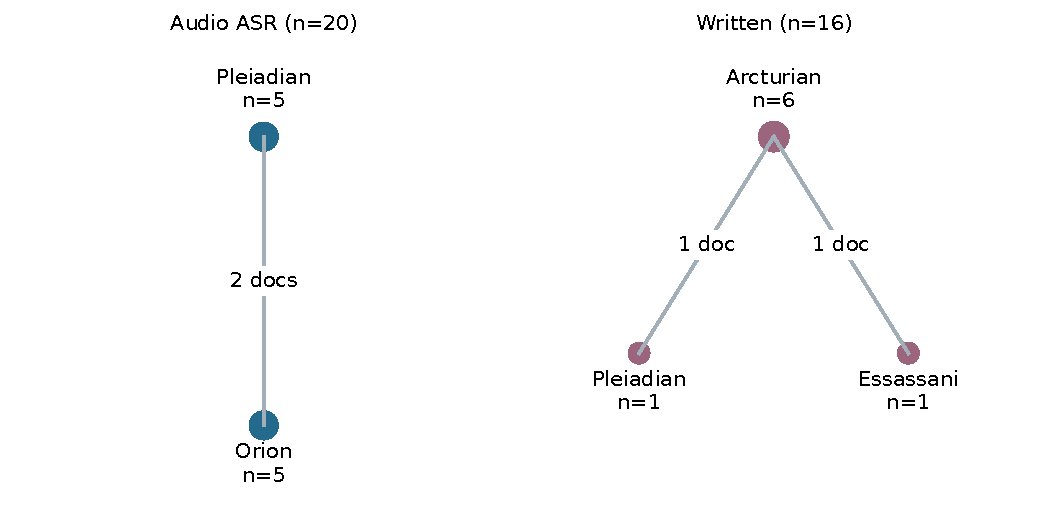
\includegraphics[width=\textwidth]{generated/figures/civilization-mentions.pdf}
\caption{Nodes are explicit claimed-civilization/star-system dictionary families and labels give documents with at least one match. Edge labels give documents mentioning both families once per pair; audio and publisher-text panels remain separate. Zero-hit families are omitted from the drawing and retained in the complete count table. Positions are schematic. Star-system/Orion mentions can concern astronomy or fiction; ASR variants are not fuzzy-corrected. Bashar and Ashtar entity names are recorded separately and are not silently mapped to a civilization.}
\label{fig:civilization-mentions}
\end{figure*}


\begin{figure*}[t]
\centering
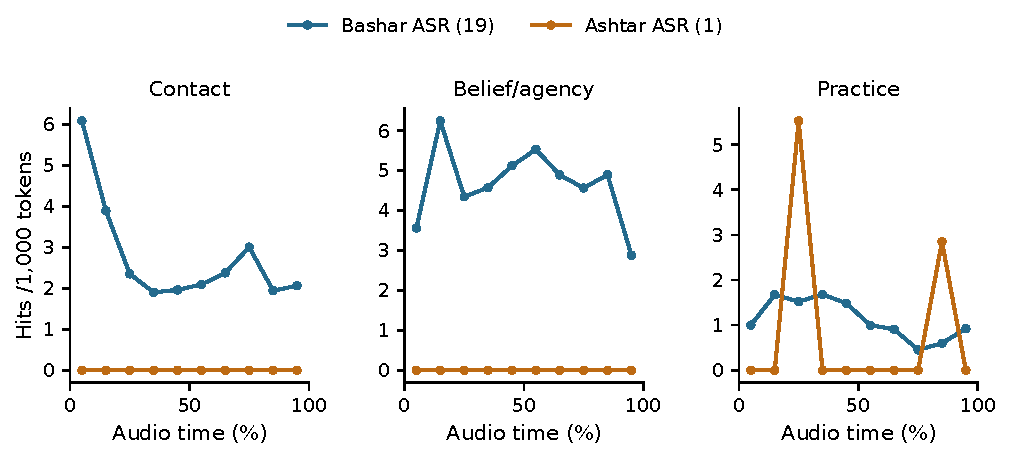
\includegraphics[width=\textwidth]{generated/figures/audio-time-profiles.pdf}
\caption{Segments are assigned by their midpoint to ten equal decoded-audio-time bins. Each bin's keyword occurrences are divided by its own common-token denominator; curves are equal-document means. The Ashtar curve represents one recording, not an estimated population trajectory. Bins are dependent and not independent observations; source intro/outro/advertising remains unsegmented.}
\label{fig:audio-time-profiles}
\end{figure*}


The displayed audio document graph retains 32 edges under its two-neighbor/threshold rule. The separate all-pair threshold diagnostic counts 190 possible reused-document pairs. Its edge counts vary from a complete graph at 0.15 to zero at 0.65; this diagnostic is not the same graph rule as the displayed top-two-neighbor union. Network density is therefore partly a construction choice, not a measured social connectivity.

The strict audio civilization/star-system dictionary returns only two nonzero families: Pleiadian / Pleiades: 5/20 documents, 6 mentions; Orion: 5/20 documents, 8 mentions. They co-occur in two documents. Missing strict matches do not establish absence of a topic, a correct ASR spelling or an attributed group. The authored branch has Arcturian/Arcturus matches in six documents, whereas three items carry the corresponding source label. This is a concrete difference between a source's attributed label and terms appearing in its body. Orion and other names remain potentially astronomical or fictional mentions.

A separately labeled post-hoc spelling sensitivity retains the strict counts and inspects unvalidated variants. Essassani / Sassani has 0 strict matches and 4 additional candidate-spelling occurrences across 4 source documents. Ashtar has 3 strict matches and 14 additional candidate-spelling occurrences across 1 source documents. These are ASR-string candidates, not audio-validated corrections or verified identity attributions; the primary dictionary graph is unchanged.

An executed synthetic control illustrates a stronger semantic limit: Following excitement is safe and Following excitement is not safe have cosine 1.00 in the actual audio-fitted space. They are purpose-built contrasting sentences, not a corpus prevalence or error-rate estimate. Lexical resemblance alone cannot test agreement or safety.

\subsection{Sensitivity and limits of simple removals}

Excluding declared proper-name tokens in the audio-ASR cohort gives pairwise-cosine rank correlation 0.998 with baseline and preserves 95 percent of nearest-neighbor choices. These are within-corpus perturbation results, not accuracy estimates.

Excluding the declared commercial vocabulary in the audio-ASR cohort gives pairwise-cosine rank correlation 0.998 with baseline and preserves 90 percent of nearest-neighbor choices. These are within-corpus perturbation results, not accuracy estimates.

Restricting ASR to the central 80 percent of audio time in the audio-ASR cohort gives pairwise-cosine rank correlation 0.945 with baseline and preserves 80 percent of nearest-neighbor choices. These are within-corpus perturbation results, not accuracy estimates.

The separate written commercial-vocabulary exclusion gives rank correlation 1.000 and preserves 100 percent of nearest-neighbor choices in that fitted written cohort. That unchanged result does not show that publisher promotion was absent or successfully removed.

Across the 14 publisher omissions, mean matched topic cosine is 0.789 and its minimum is 0.677. The original vocabulary and IDF stay fixed, so this isolates a different influence than refitting the entire pipeline. The high commercial-removal correlation is limited to its declared word list: protein, collagen and other product-specific words remain outside that list. Central-time restriction and lexical removal do not verify speaker or advertisement removal.

\subsection{Source-linked readings and question/answer candidates}

The model agent inspected 105 windows: 96 fixed windows plus 9 explicitly post-hoc or extended comparison windows. The 19,603 packet words include overlapping windows and are not unique corpus coverage. Deduplicated ASR coverage is 11,992/226,093 whitespace words (5.30 percent), across 1,112/21,197 segments. The written coverage is 6,319/13,656 whitespace words (46.27 percent). Both reading fractions use the same whitespace rule, which differs from the common analytical tokenizer and inherited written-source receipt counts. The lone Athina transcript and Paul extraction were read completely as text, while the other audio records were sampled. This asymmetric reading depth is a limitation of qualitative context comparisons. Full computational use of a transcript is not full semantic reading.

Ten provisional codes yield 142 source--code assignments supported by inspected windows. The model-assisted publisher-promotion code occurs in selected windows of 15/20 audio records and 15/16 written records. Those selected-window source-presence counts are not a population advertising rate. They also differ from a narrow commercial-word dictionary: a source can promote a book or product without matching that dictionary.

The candidate database contains 37 records in 10 provisional prompt families. Of these, 16 are analyst-constructed comparison prompts for written sources, not questions observed in an interaction. The 21 audio question-like candidates comprise 14 explicit interview-prompt candidates, one fragmentary interview prompt and six rhetorical, self-question or secondary-report candidates. They retain unsegmented question/answer turns and unknown speaker attribution. Shared family membership does not establish equivalent prompts or agreement.

The readings provide competing interpretations for numerical resemblance. A skeptical Ross/Carrie passage uses belief/reality vocabulary to criticize the guidance, whereas an Align middle window contains a retail advertisement. A Gateways reply qualifies agency rather than presenting it as literally unconstrained. The full Athina ASR separates a creator introduction, a source-framed address and closing reflection, and discusses a staged life-purpose account. Its NMF words workers, jumps and sole are interpreted in that spiritual/ASR context; the last is a potential soul homophone, not a validated correction. These paraphrases are model-agent interpretations with retained locators, not verified speaker testimony or independent human coding.

The following six case comparisons describe the actual selected material. They are interpretive findings of this window-reading exercise; differences in prompts and source formats prevent population or agreement conclusions.

\paragraph{Shared words can accompany explicit disagreement} The skeptical source restates belief/reality guidance while criticizing its repetition and ambiguity. A similarity edge to an interview therefore cannot be interpreted as agreement. Support: A16 3633.59--3693.91s.

\paragraph{Advertising and publisher framing are present in sampled source bodies} Retail advertising occurs in the temporal middle of one interview; health-service and software promotions bracket two others, and a podcast advertisement interrupts a brief organizational-role answer. Untreated document topics can therefore describe publishing infrastructure. Support: A03 2533.66--2567.74s; A01 0.00--30.16s; A02 6028.66--6062.80s; A13 1938.38--2002.82s.

\paragraph{Broad agency and future-contact themes include qualifications} One source limits changes to an earthly-life framework, another refuses to treat rapid developments as a settled forecast, and another portrays a contact forecast as conditional and potentially influenced by attention to it. These distinctions would disappear in a simple shared-keyword count. Support: A08 349.58--410.28s; A15 272.06--334.46s; A12 293.05--359.93s.

\paragraph{A singleton component needs source-level interpretation} In the Ashtar-attributed recording, workers belongs to the spiritual compound lightworkers, jumps describes claimed timeline/vibration changes, and sole occurs where surrounding text suggests a possible recognition error involving soul. These observations explain how a component can combine genuine source-specific vocabulary and transcription noise. Support: A18 113.70--138.50s; A18 348.88--455.66s; A18 846.20--876.90s.

\paragraph{A broad question family does not make answers equivalent} Contact-readiness passages address different subjects: an individual preparing for an encounter, a collective described as unready, and a selected audience described as already prepared. Their shared theme is not enough to establish agreement or contradiction. Support: A20 2676.51--2737.95s; T08 opening 250 words; T03 opening 250 words.

\paragraph{Practical guidance has different forms across the available sources} The Bashar-context exchange clarifies a general action-and-belief formula, while the complete single Ashtar comparison presents accepting, identifying and embodying a life purpose. Paul Selig and the Daniel posts offer additional spiritual framings, but these source types are not balanced evidence about separate civilizations. Support: A11 166.06--229.94s; A18 1095.10--1435.55s; T16 full text; T10 opening 250 words.
